%% =====================================================================
%%  Confidence-Gated Dual-Process Fall Detection (RCDP)
%%  Target journal: IEEE Journal of Biomedical and Health Informatics
%%
%%  Build:  pdflatex main -> bibtex main -> pdflatex main -> pdflatex main
%%          (or: tectonic main.tex)
%%
%%  Layout:  tables/      one .tex per table, \input from this file
%%           figures/     TikZ sources (.tex) and rendered plots (.pdf)
%%           algorithms/  algorithm floats
%%           results_text/ counts CSVs + DATA_LOCK.txt
%%           configs/     locked YAML protocol snapshots
%%           prompts/     system prompts + evidence serializer template
%%
%%  BEFORE SUBMISSION: resolve and delete every \authorcheck{...} marker
%%  (search for "authorcheck"); then make \authorcheck expand to nothing
%%  or remove the macro. Red text must not reach the submitted PDF.
%% =====================================================================
\documentclass[journal]{IEEEtran}

\usepackage{amsmath,amssymb,amsfonts}
\usepackage{graphicx}
\usepackage{booktabs}
\usepackage{array}
\usepackage{multirow}
\usepackage{cite}
\usepackage{url}
\usepackage{xcolor}
\usepackage{tikz}
\usetikzlibrary{arrows.meta,positioning,fit,calc}
\usepackage{algorithm}
\usepackage{algorithmic}
\usepackage[hidelinks]{hyperref}

\newtheorem{proposition}{Proposition}
\newcommand{\proofpar}[1]{\par\noindent\textit{Proof.} #1\hfill$\blacksquare$\par\medskip}
% Items the authors must verify against the experiment code before submission.
% Markers resolved for A1–A6 / figure; remaining placeholders are empty (fill AUTHORS before submit).
\newcommand{\authorcheck}[1]{}

\begin{document}

\title{Confidence-Gated Dual-Process Fall Detection:\\
Retrieval-Augmented Reasoning and Cost-Sensitive\\
Response on Wearable Inertial Sensor Data}

\author{Harshal Dharpure\\
Indian Institute of Technology Patna\\
\texttt{harshal\_2511ai30@iitp.ac.in}\\
ORCID: not available}

\maketitle

% =====================================================================
\begin{abstract}
Wearable fall detectors must trade missed falls against false alarms, and their errors concentrate on everyday movements that resemble falls. This study evaluates a confidence-gated decision layer around a fixed detector under a sensor-only protocol. A frozen convolutional, recurrent and attention-based detector scores every sensor window. A two-threshold confidence gate, calibrated under a cost that weights a missed fall ten times a false alarm, decides confident windows directly and escalates ambiguous ones to a deliberative path that summarises biomechanical evidence, retrieves similar training cases and queries a locally hosted language model. In five subject-independent SisFall folds, the best blend achieved F1 $0.772\pm0.025$ versus $0.768\pm0.019$ for the frozen detector, with expected cost $1079.6\pm115.3$ versus $1086.6\pm80.6$. Event-level and prospective free-living validation remain necessary.
\end{abstract}

\begin{IEEEkeywords}
Clinical decision support, confidence gating, cost-sensitive learning, fall detection, large language models, retrieval-augmented reasoning, selective prediction, wearable inertial sensors.
\end{IEEEkeywords}

% =====================================================================
\section{Introduction}
\label{sec:intro}

\IEEEPARstart{F}{alls} are the second leading cause of unintentional-injury death worldwide, with an estimated $684{,}000$ fatalities and $37.3$ million falls requiring medical attention each year; death rates are highest above age~60~\cite{who2021falls}. Time spent on the floor unable to summon help---the \emph{long lie}---is independently associated with hospitalisation and institutionalisation~\cite{fleming2008longlie,tinetti1997falls}. Wearable inertial measurement units (IMUs) are therefore attractive for continuous home monitoring~\cite{iglesias2019wearable,nurek2020fallsurvey,khan2017review,sisfall2017}, and deep detectors now report strong benchmark accuracy~\cite{ren2021survey,mubashir2013survey}.

Three gaps remain. \emph{First}, stumbles and compensatory recoveries can resemble falls in wearable signals~\cite{aziz2016fall,aziz2012nearfall,aziz2014causes}. We therefore evaluate a stress set containing stumbles, non-fall movements, falls, and other ADLs. \emph{Second}, softmax scores are a poor basis for deferral: modern networks are miscalibrated~\cite{guo2017calibration,lakshminarayanan2017ensembles}, and the decision to abstain needs its own risk analysis~\cite{chow1970reject,el2010foundations,geifman2017selective,cortes2016rejection}. \emph{Third}, a fall/ADL bit is not a response: dispatch, caregiver notification, monitoring and logging carry unequal costs, and missed falls dominate risk~\cite{elkan2001foundations,noury2008evaluation}.

Bhatti \textit{et al.}~\cite{bhatti2025beyond} present a hybrid CNN--LSTM--Attention detector for multi-phase fall analysis. That line of work optimises the detector. We ask a different question: \emph{holding the detector fixed, can a decision layer raise recall and lower expected response cost on the hard cases?} Our answer is the Risk-Calibrated Dual-Process (RCDP) pipeline (Fig.~\ref{fig:arch}). System~1 is the frozen primary detector plus a dual-threshold gate. System~2 handles only ambiguous windows: it serialises biomechanical evidence, retrieves labelled training cases~\cite{minilm2020,lewis2020rag}, queries a local language model~\cite{wei2022cot,yao2023react,ollama,mistral2023} and emits a simulated graded response. Classification is scored under
\begin{equation}
\mathcal{R}_\beta = \beta\cdot\mathrm{FN}+\mathrm{FP},\qquad \beta=10.
\label{eq:risk}
\end{equation}

\paragraph{Contributions}
\begin{itemize}
\item A selective-risk decomposition (Prop.~\ref{prop:defer}) stating when escalation to an adjudicator lowers risk with edge decisions held fixed.
\item A dual-process decision layer---gate, evidence, retrieval, local reasoning, simulated action---around a primary detector whose weights are never updated (Fig.~\ref{fig:arch}, Algs.~\ref{alg:rcdp}--\ref{alg:gate}).
\item A subject-independent evaluation on SisFall (main and stress sets) and KFall (binary and stress sets), with a second backbone, a $2{\times}2$ retrieval/reasoner ablation, a cost-derived threshold control and constant-prediction controls.
\item Two negative results: retrieval or reasoning alone does not reproduce the gain, and a critic permitted to overturn fall labels multiplies missed falls.
\end{itemize}
All gains are measured against the \emph{same} primary-detector checkpoints under our protocol; we do not compare with the published multi-phase KFall results of~\cite{bhatti2025beyond}, which use a different protocol and label granularity.

% =====================================================================
\section{Related Work}
\label{sec:related}

Table~\ref{tab:related} positions RCDP against adjacent literature families.

\begin{table*}[!t]
\centering
\caption{Conceptual positioning against selected adjacent literature families. The comparison motivates the evaluated combination of deferral, retrieved evidence, language-model adjudication and simulated response; it is not an exhaustive novelty search or evidence that no prior system combines these elements.}
\label{tab:related}
\renewcommand{\arraystretch}{1.15}
\newcolumntype{L}[1]{>{\raggedright\arraybackslash}p{#1}}
\begin{tabular}{@{}L{0.155\linewidth} L{0.13\linewidth} L{0.13\linewidth} L{0.13\linewidth} L{0.13\linewidth} L{0.13\linewidth}@{}}
\toprule
Family & Uncertainty handling & Explanation & Response policy & Near-fall protocol & Asymmetric cost \\
\midrule
Threshold rules~\cite{bourke2007threshold,nurek2020fallsurvey}
 & fixed magnitude cut & rule trace & binary alarm & no & implicit \\
Deep IMU detectors~\cite{bhatti2025beyond,kfall2021,ren2021survey}
 & softmax score & attention maps & none & partial (phase labels) & no \\
Selective prediction / learning to defer~\cite{chow1970reject,geifman2017selective,cortes2016rejection,mozannar2020defer}
 & learned reject function & none & none & no & optional \\
Split conformal prediction~\cite{vovk2005algorithmic,angelopoulos2023gentle}
 & coverage-controlled sets & none & none & no & no \\
LLMs over raw sensor data~\cite{ji2024hargpt,li2024sensorllm,kim2024healthllm}
 & prompt confidence & natural-language rationale & none & no & no \\
\midrule
\textbf{RCDP (this work)}
 & \textbf{cost-calibrated dual threshold}
 & \textbf{biomechanical evidence $+$ retrieved cases $+$ rationale}
 & \textbf{graded action agent}
 & \textbf{Near-fall stress benchmark}
 & \textbf{$\mathcal{R}_\beta$, $\beta{=}10$} \\
\bottomrule
\end{tabular}
\end{table*}


\subsection{Wearable Fall Detection}
Threshold rules on acceleration magnitude~\cite{bourke2007threshold,nurek2020fallsurvey} gave way to classical learners and then to CNN, LSTM, TCN and Transformer models evaluated on SisFall~\cite{sisfall2017}, KFall~\cite{kfall2021}, UP-Fall~\cite{martinez2019upfall}, UniMiB SHAR~\cite{micucci2017unimib} and FallAllD~\cite{saleh2021fallalld}. Surveys identify the free-living trade-off between sensitivity and nuisance alarms as the unsolved problem~\cite{iglesias2019wearable,khan2017review,ren2021survey,mubashir2013survey}, and Noury \textit{et al.}~\cite{noury2008evaluation} argue that detectors should be evaluated under a declared cost and protocol. We reuse the CNN--LSTM--Attention motif of~\cite{bhatti2025beyond} as the primary detector and place the novelty at decision time.

\subsection{Selective Prediction and Deferral}
Classification with a reject option dates to Chow~\cite{chow1970reject} and has been developed into selective classification~\cite{el2010foundations,geifman2017selective}, learning with rejection~\cite{cortes2016rejection} and learning to defer to an expert~\cite{madras2018defer,mozannar2020defer}. Calibration is a prerequisite for thresholding scores~\cite{guo2017calibration,platt1999probabilistic}. Our gate is a post-hoc, cost-calibrated member of this family; we do not train a joint predictor--rejector because the detector is fixed by design. Split conformal prediction~\cite{vovk2005algorithmic,shafer2008tutorial,angelopoulos2023gentle,romano2019conformalized} offers set-valued alternatives, but its marginal guarantee requires exchangeability, which subject shift and overlapping windows violate; we leave it to future work. Cost-sensitive learning follows Elkan~\cite{elkan2001foundations}.

\subsection{Language Models over Sensor Data}
Retrieval-augmented generation~\cite{lewis2020rag} with compact sentence encoders~\cite{minilm2020,reimers2019sbert} supports case-based prompting; chain-of-thought~\cite{wei2022cot}, reason--act loops~\cite{yao2023react} and self-refinement~\cite{madaan2023selfrefine} structure decisions. HARGPT reads raw IMU streams zero-shot~\cite{ji2024hargpt}, SensorLLM aligns sensor channels with text~\cite{li2024sensorllm} and Health-LLM predicts health outcomes from wearable data~\cite{kim2024healthllm}. We differ in two ways: the model receives a serialised evidence string rather than raw signals, which limits but does not remove the risk of unsupported rationales~\cite{huang2025hallucination,singhal2023medpalm}; and it is invoked only on the ambiguous band under an explicit clinical cost.

% =====================================================================
\section{Problem Formulation}
\label{sec:problem}

Let $(\mathbf{x},y)\sim P$ over $\mathcal{X}\times\{0,1\}$, where $\mathbf{x}\in\mathbb{R}^{C\times T}$ is an inertial window and $y{=}1$ denotes a fall. The asymmetric loss is
\begin{equation}
\ell_\beta(\hat{y},y)=\beta\cdot\mathbf{1}\{\hat{y}{=}0,y{=}1\}+\mathbf{1}\{\hat{y}{=}1,y{=}0\},
\label{eq:loss}
\end{equation}
the population form of~\eqref{eq:risk}. A \emph{selective decision system} $(f,g,h)$ comprises a frozen scorer $f:\mathcal{X}\to[0,1]$ producing $p(\mathbf{x})$, a gate $g:[0,1]\to\{\textsf{edge},\textsf{defer}\}$ and an adjudicator $h:\mathcal{X}\to\{0,1\}$ invoked only on deferral. Each deferral costs $\lambda\ge 0$ (compute, energy, latency). The system risk is
\begin{multline}
\mathcal{R}(f,g,h)=\mathbb{E}\big[\mathbf{1}\{g{=}\textsf{edge}\}\,\ell_\beta(\hat{y}_f(\mathbf{x}),y)\big]\\
+\;\mathbb{E}\big[\mathbf{1}\{g{=}\textsf{defer}\}\,(\ell_\beta(h(\mathbf{x}),y)+\lambda)\big].
\label{eq:selrisk}
\end{multline}

\begin{proposition}[Hard-decision Bayes threshold]
\label{prop:bayes}
If $p$ is calibrated and the system never defers, the risk-minimising rule is $\hat{y}=\mathbf{1}\{p(\mathbf{x})\ge\tau^\ast\}$ with
\begin{equation}
\tau^{\ast}=\frac{1}{\beta+1}=\frac{1}{11}\approx 0.091 .
\label{eq:tau_star}
\end{equation}
\end{proposition}
\proofpar{Given $p$, predicting $1$ costs $(1-p)$ in expectation and predicting $0$ costs $\beta p$; predict $1$ iff $p\ge 1/(\beta{+}1)$.}

Let the gate be the dual-threshold rule~\eqref{eq:gate} and let $\mathcal{A}=\{\mathbf{x}:\tau_{\mathrm{low}}<p(\mathbf{x})<\tau_{\mathrm{high}}\}$ be the ambiguous band, with mass $\pi=\Pr(\mathbf{x}\in\mathcal{A})$ (the escalation rate).

\begin{proposition}[When deferral is worthwhile]
\label{prop:defer}
Assume $\pi>0$. Let $r_1=\mathbb{E}[\ell_\beta(\hat{y}_f(\mathbf{x}),y)\mid\mathbf{x}\in\mathcal{A}]$ and $r_2=\mathbb{E}[\ell_\beta(h(\mathbf{x}),y)\mid\mathbf{x}\in\mathcal{A}]$ be the band risks of the primary detector and the adjudicator, and let $\mathcal{R}_{\mathrm{fb}}$ be the risk of the same edge decisions with the primary-detector rule inside $\mathcal{A}$ and no deferral charge. Then
\begin{equation}
\mathcal{R}(f,g,h)-\mathcal{R}_{\mathrm{fb}}=\pi\,\big(r_2-r_1+\lambda\big),
\label{eq:deferdelta}
\end{equation}
so escalation strictly reduces risk iff $r_1-r_2>\lambda$.
\end{proposition}
\proofpar{Both systems agree outside $\mathcal{A}$; inside, the fallback incurs $r_1$ and the deferring system $r_2+\lambda$.}

Three consequences organise the experiments. (i)~\emph{The gate alone cannot
help} if the deferred rule equals the primary-detector rule. (ii)~\emph{The
decision layer must be compared under the declared cost} on shared test cases.
(iii)~\emph{$\pi$ scales the benefit but not its sign}, so escalation rate is
reported separately. The calibration objective (Alg.~\ref{alg:gate}) scores
only edge decisions plus a deferral penalty; it is a routing surrogate rather
than a direct minimisation of~\eqref{eq:selrisk}, and reported classification
costs exclude $\lambda$.

% =====================================================================
\section{Method}
\label{sec:method}

Fig.~\ref{fig:arch} and Alg.~\ref{alg:rcdp} summarise the pipeline; block numbers below refer to Fig.~\ref{fig:arch}.

\begin{figure*}[!t]
\centering
\resizebox{\linewidth}{!}{% ---------------------------------------------------------------------
% Fig. 1 -- RCDP architecture (dual-process view). Vector TikZ.
% Requires tikz libraries arrows.meta, positioning, fit, calc.
% Designed for figure*; wrap with \resizebox{\linewidth}{!}{...}.
% Numbered blocks 1, 2, 3, 3a--3e, 4, 5 are referenced in the text.
% ---------------------------------------------------------------------
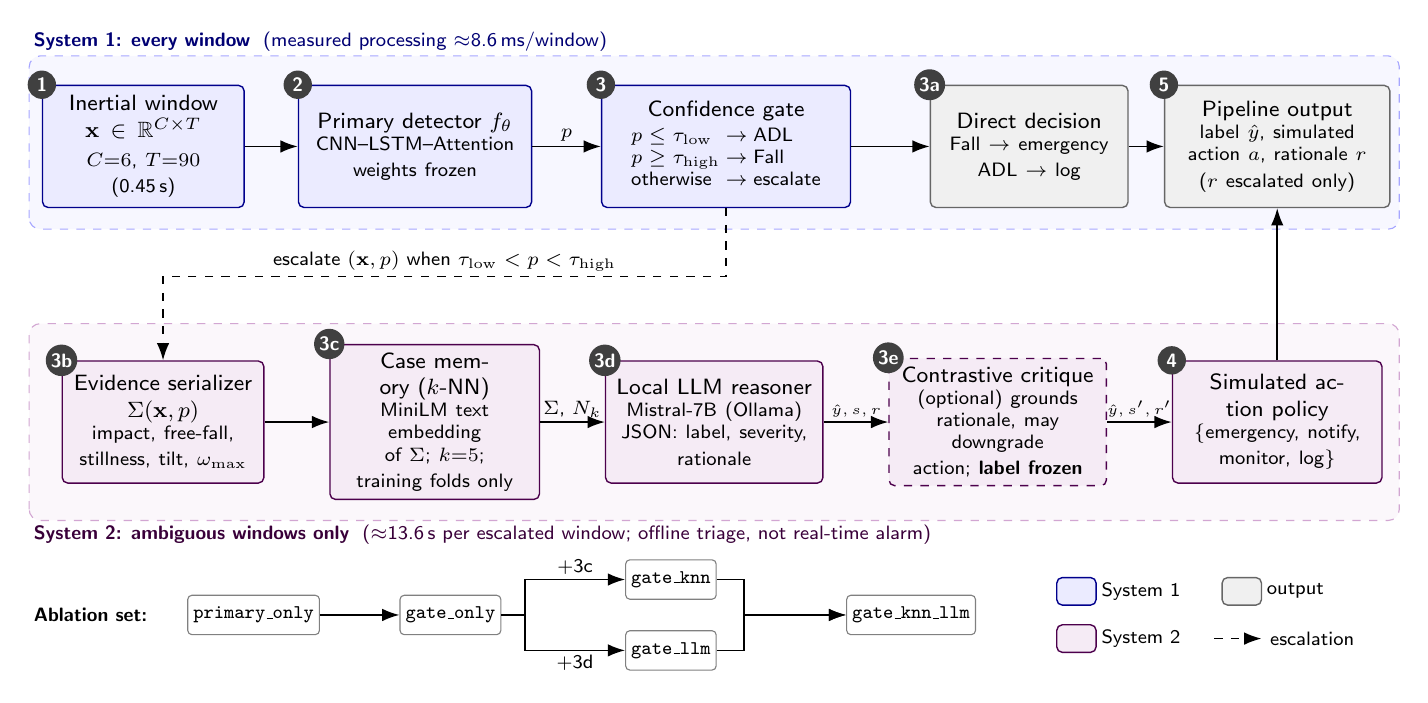
\begin{tikzpicture}[
  font=\footnotesize\sffamily,
  s1/.style={draw=blue!55!black, line width=0.5pt, rounded corners=2pt,
             fill=blue!8, align=center, inner sep=3pt, minimum height=1.55cm},
  s2/.style={draw=violet!60!black, line width=0.5pt, rounded corners=2pt,
             fill=violet!8, align=center, inner sep=3pt, minimum height=1.55cm},
  opt/.style={s2, dashed},
  outbox/.style={draw=black!60, line width=0.5pt, rounded corners=2pt,
             fill=black!6, align=center, inner sep=3pt, minimum height=1.55cm},
  badge/.style={circle, fill=black!75, text=white, font=\scriptsize\sffamily\bfseries,
             inner sep=0.8pt, minimum size=3.6mm},
  arr/.style={-{Latex[length=2.2mm,width=1.6mm]}, line width=0.6pt},
  darr/.style={-{Latex[length=2.2mm,width=1.6mm]}, line width=0.6pt, dashed},
  lbl/.style={font=\scriptsize\sffamily, inner sep=1.5pt},
  mode/.style={draw=black!50, rounded corners=1.5pt, fill=white,
             font=\scriptsize\ttfamily, inner sep=2pt, minimum height=0.5cm}
]

% ---------- backdrops ----------
\draw[draw=blue!35, dashed, rounded corners=4pt, fill=blue!3]
  (-0.10,-1.05) rectangle (17.30,1.15);
\draw[draw=violet!35, dashed, rounded corners=4pt, fill=violet!3]
  (-0.10,-4.75) rectangle (17.30,-2.25);
\node[lbl, anchor=south west, text=blue!45!black] at (-0.10,1.15)
  {\textbf{System 1: every window}\; (measured processing $\approx$8.6\,ms/window)};
\node[lbl, anchor=north west, text=violet!45!black] at (-0.10,-4.75)
  {\textbf{System 2: ambiguous windows only}\; ($\approx$13.6\,s per escalated window; offline triage, not real-time alarm)};

% ---------- System 1 row ----------
\node[s1, text width=2.35cm] (in) at (1.35,0)
  {Inertial window\\$\mathbf{x}\in\mathbb{R}^{C\times T}$\\[1pt]\scriptsize $C{=}6$, $T{=}90$ (0.45\,s)};
\node[s1, text width=2.75cm] (det) at (4.80,0)
  {Primary detector $f_\theta$\\\scriptsize CNN--LSTM--Attention\\\scriptsize weights frozen};
\node[s1, text width=2.95cm] (gate) at (8.75,0)
  {Confidence gate\\[1pt]\scriptsize
   \begin{tabular}{@{}l@{\;$\rightarrow$\;}l@{}}
   $p\le\tau_{\mathrm{low}}$ & ADL\\
   $p\ge\tau_{\mathrm{high}}$ & Fall\\
   otherwise & escalate
   \end{tabular}};
\node[outbox, text width=2.30cm] (direct) at (12.60,0)
  {Direct decision\\\scriptsize Fall $\rightarrow$ emergency\\\scriptsize ADL $\rightarrow$ log};
\node[outbox, text width=2.65cm] (outp) at (15.75,0)
  {Pipeline output\\\scriptsize label $\hat{y}$, simulated\\\scriptsize action $a$, rationale $r$\\\scriptsize ($r$ escalated only)};

\node[badge] at (in.north west)     {1};
\node[badge] at (det.north west)    {2};
\node[badge] at (gate.north west)   {3};
\node[badge] at (direct.north west) {3a};
\node[badge] at (outp.north west)   {5};

\draw[arr] (in) -- (det);
\draw[arr] (det) -- node[lbl, above] {$p$} (gate);
\draw[arr] (gate) -- (direct);
\draw[arr] (direct) -- (outp);

% ---------- System 2 row ----------
\node[s2, text width=2.35cm] (ev) at (1.60,-3.50)
  {Evidence serializer\\$\Sigma(\mathbf{x},p)$\\\scriptsize impact, free-fall,\\\scriptsize stillness, tilt, $\omega_{\max}$};
\node[s2, text width=2.45cm] (knn) at (5.05,-3.50)
  {Case memory ($k$-NN)\\\scriptsize MiniLM text embedding\\\scriptsize of $\Sigma$; $k{=}5$;\\\scriptsize training folds only};
\node[s2, text width=2.55cm] (llm) at (8.60,-3.50)
  {Local LLM reasoner\\\scriptsize Mistral-7B (Ollama)\\\scriptsize JSON: label, severity,\\\scriptsize rationale};
\node[opt, text width=2.55cm] (crit) at (12.20,-3.50)
  {Contrastive critique\\\scriptsize (optional) grounds\\\scriptsize rationale, may downgrade\\\scriptsize action; \textbf{label frozen}};
\node[s2, text width=2.45cm] (act) at (15.75,-3.50)
  {Simulated action policy\\\scriptsize \{emergency, notify,\\\scriptsize monitor, log\}};

\node[badge] at (ev.north west)   {3b};
\node[badge] at (knn.north west)  {3c};
\node[badge] at (llm.north west)  {3d};
\node[badge] at (crit.north west) {3e};
\node[badge] at (act.north west)  {4};

\draw[darr] (gate.south) -- (8.75,-1.65) -| node[lbl, pos=0.25, above]
  {escalate $(\mathbf{x},p)$ when $\tau_{\mathrm{low}}<p<\tau_{\mathrm{high}}$} (ev.north);
\draw[arr] (ev) -- (knn);
\draw[arr] (knn) -- node[lbl, above] {$\Sigma$, $N_k$} (llm);
\draw[arr] (llm) -- node[lbl, above, font=\tiny] {$\hat{y},s,r$} (crit);
\draw[arr] (crit) -- node[lbl, above, font=\tiny] {$\hat{y},s',r'$} (act);
\draw[arr] (act) -- (outp);

% ---------- footer: ablation set (2x2 design) and legend ----------
\node[lbl, anchor=west] at (-0.10,-5.95) {\textbf{Ablation set:}};
\node[mode] (m0) at (2.75,-5.95) {primary\_only};
\node[mode] (m1) at (5.25,-5.95) {gate\_only};
\node[mode] (m2) at (8.05,-5.50) {gate\_knn};
\node[mode] (m3) at (8.05,-6.40) {gate\_llm};
\node[mode] (m4) at (11.10,-5.95) {gate\_knn\_llm};
\draw[arr] (m0) -- (m1);
\draw[arr] (m1.east) -- ++(0.30,0) |- node[lbl, pos=0.75, above] {+3c} (m2.west);
\draw[arr] (m1.east) -- ++(0.30,0) |- node[lbl, pos=0.75, below] {+3d} (m3.west);
\draw[arr] (m2.east) -- ++(0.35,0) |- (m4.west);
\draw[arr] (m3.east) -- ++(0.35,0) |- (m4.west);

\node[s1, minimum height=0.35cm, minimum width=0.5cm] (lg1) at (13.20,-5.65) {};
\node[lbl, anchor=west] at (lg1.east) {System 1};
\node[s2, minimum height=0.35cm, minimum width=0.5cm] (lg2) at (13.20,-6.25) {};
\node[lbl, anchor=west] at (lg2.east) {System 2};
\node[outbox, minimum height=0.35cm, minimum width=0.5cm] (lg3) at (15.30,-5.65) {};
\node[lbl, anchor=west] at (lg3.east) {output};
\draw[darr] (14.95,-6.25) -- (15.55,-6.25);
\node[lbl, anchor=west] at (15.60,-6.25) {escalation};

\end{tikzpicture}
}
\caption{RCDP architecture. Every window passes the frozen primary detector (2)
and confidence gate (3); confident windows are decided directly (3a). Only
windows with $\tau_{\mathrm{low}}<p<\tau_{\mathrm{high}}$ enter the
deliberative path: evidence serialisation (3b), case retrieval (3c), local
reasoning (3d), and a simulated action policy (4).}
\label{fig:arch}
\end{figure*}

\begin{algorithm}[!t]
\caption{RCDP inference for one inertial window}
\label{alg:rcdp}
\begin{algorithmic}[1]
\REQUIRE Window $\mathbf{x}\in\mathbb{R}^{C\times T}$; frozen primary detector $f_\theta$; gate $(\tau_{\mathrm{low}},\tau_{\mathrm{high}})$; case memory $\mathcal{M}$; reasoner $\mathcal{L}$; optional critique $\mathcal{C}$; action policy $\mathcal{A}$; width $k$
\STATE $p\leftarrow \mathrm{softmax}(f_\theta(\mathbf{x}))_1$ \COMMENT{block 2; no weight update}
\STATE $r\leftarrow\varnothing$
\IF{$p\le\tau_{\mathrm{low}}$}
  \STATE $\hat{y}\leftarrow\mathrm{ADL}$; \; $a\leftarrow\texttt{log}$ \COMMENT{block 3a}
\ELSIF{$p\ge\tau_{\mathrm{high}}$}
  \STATE $\hat{y}\leftarrow\mathrm{Fall}$; \; $a\leftarrow\texttt{emergency}$ \COMMENT{block 3a}
\ELSE
  \STATE $\Sigma\leftarrow\textsc{SerializeEvidence}(\mathbf{x},p)$ \COMMENT{block 3b}
  \STATE $N_k\leftarrow\textsc{TopK}(\mathcal{M},\Sigma,k)$ \COMMENT{block 3c, \eqref{eq:cosine}}
  \STATE $(\hat{y},s,r)\leftarrow\mathcal{L}(\Sigma,N_k)$ \COMMENT{block 3d}
  \STATE $(s,r)\leftarrow\mathcal{C}(\hat{y},s,r,\Sigma)$ \COMMENT{block 3e; $\hat{y}$ immutable}
  \STATE $a\leftarrow\mathcal{A}(\hat{y},s,\Sigma)$ \COMMENT{block 4, simulated}
\ENDIF
\STATE \textbf{return} $(\hat{y},a,r)$ \COMMENT{block 5}
\end{algorithmic}
\end{algorithm}


\subsection{Primary Detector (Block 2)}
Let $\mathbf{x}\in\mathbb{R}^{C\times T}$ be an inertial window ($C{=}6$, $T{=}90$ on SisFall). A CNN--LSTM--Attention backbone $f_\theta$ following~\cite{bhatti2025beyond} maps $\mathbf{x}$ to logits $\boldsymbol{\ell}\in\mathbb{R}^{2}$ and
\begin{equation}
p = \hat{p}_\theta(y{=}1\mid\mathbf{x}) = \frac{e^{\ell_1}}{e^{\ell_0}+e^{\ell_1}}.
\label{eq:pfall}
\end{equation}
Its weights are frozen at inference; the baseline mode \texttt{primary\_only} decides with a single calibrated threshold. For context we trained a reference zoo (CNN1D, LSTM, CNN--LSTM, TCN~\cite{bai2018tcn}, ModernTCN~\cite{iglesias2023modern}, TSMixer~\cite{tsmixer2023}, PatchTST~\cite{patchtst2023}, Transformer~\cite{vaswani2017attention}; Supplementary Table~S1) and repeated the full stack with HARMamba~\cite{li2025harmamba}, a bidirectional state-space activity-recognition backbone with about $0.6\times$ the parameters ($\approx$325k vs.\ $\approx$565k).

\subsection{Confidence Gate (Blocks 3, 3a)}
A dual-threshold gate routes windows:
\begin{equation}
\mathrm{route}(p)=
\begin{cases}
\mathrm{ADL}\ (\texttt{log}), & p \le \tau_{\mathrm{low}},\\
\mathrm{Fall}\ (\texttt{emergency}), & p \ge \tau_{\mathrm{high}},\\
\mathrm{escalate}, & \text{otherwise.}
\end{cases}
\label{eq:gate}
\end{equation}
Thresholds are fit by grid search on subject-held-out calibration windows (Alg.~\ref{alg:gate}). Under FN-heavy cost, $\tau_{\mathrm{low}}$ is pushed towards zero and both $\tau^\ast$ and $0.5$ fall inside the band (Fig.~\ref{fig:gateband}).

\begin{figure}[!t]
\centering
\resizebox{\linewidth}{!}{% ---------------------------------------------------------------------
% Fig. 2 -- Decision geometry of the cost-calibrated dual-threshold gate.
% Pure TikZ. Thresholds shown are the pooled minimum-cost operating
% point of Table~\ref{tab:pareto} (tau_low = 0.05, tau_high = 0.60).
% Wrap with \resizebox{\linewidth}{!}{...} in main.tex.
% ---------------------------------------------------------------------
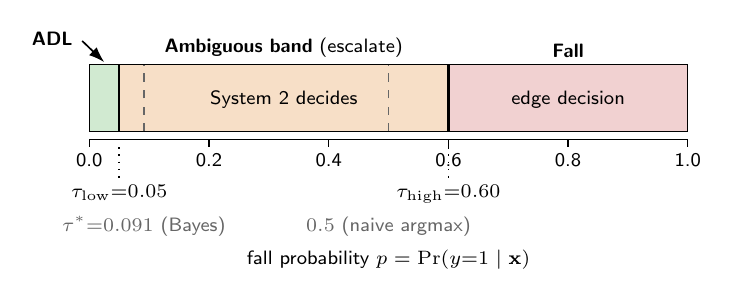
\begin{tikzpicture}[
  font=\footnotesize\sffamily,
  x=7.60cm, y=1cm,
  lbl/.style={font=\scriptsize\sffamily, inner sep=1.5pt},
  tick/.style={line width=0.5pt},
  arr/.style={-{Latex[length=2.0mm,width=1.4mm]}, line width=0.6pt}
]

% ---------- routing bands ----------
\fill[green!55!black, fill opacity=0.18] (0.00,0.00) rectangle (0.05,0.85);
\fill[orange!85!black, fill opacity=0.22] (0.05,0.00) rectangle (0.60,0.85);
\fill[red!70!black, fill opacity=0.18]    (0.60,0.00) rectangle (1.00,0.85);
\draw[line width=0.5pt] (0.00,0.00) rectangle (1.00,0.85);
\draw[line width=0.8pt] (0.05,0.00) -- (0.05,0.85);
\draw[line width=0.8pt] (0.60,0.00) -- (0.60,0.85);

% ---------- reference thresholds (inside band) ----------
\draw[dashed, line width=0.6pt, black!60] (0.091,0.00) -- (0.091,0.85);
\draw[dashed, line width=0.6pt, black!60] (0.500,0.00) -- (0.500,0.85);

% ---------- region names ----------
\node[lbl, anchor=south] at (0.325,0.88) {\textbf{Ambiguous band} (escalate)};
\node[lbl, anchor=south] at (0.800,0.88) {\textbf{Fall}};
\node[lbl, anchor=east]  at (-0.02,1.18) {\textbf{ADL}};
\draw[arr] (-0.012,1.15) -- (0.025,0.88);

\node[lbl] at (0.325,0.40) {System 2 decides};
\node[lbl] at (0.800,0.40) {edge decision};

% ---------- probability axis ----------
\draw[tick] (0.00,-0.10) -- (1.00,-0.10);
\foreach \p in {0.0,0.2,0.4,0.6,0.8,1.0}{%
  \draw[tick] (\p,-0.10) -- (\p,-0.20);
  \node[lbl, anchor=north] at (\p,-0.22) {\p};
}

% ---------- calibrated thresholds ----------
\draw[dotted, line width=0.6pt] (0.05,-0.20) -- (0.05,-0.60);
\draw[dotted, line width=0.6pt] (0.60,-0.20) -- (0.60,-0.60);
\node[lbl, anchor=north] at (0.05,-0.62) {$\tau_{\mathrm{low}}{=}0.05$};
\node[lbl, anchor=north] at (0.60,-0.62) {$\tau_{\mathrm{high}}{=}0.60$};

% ---------- reference threshold labels ----------
\node[lbl, anchor=north, text=black!60] at (0.091,-1.02) {$\tau^\ast{=}0.091$ (Bayes)};
\node[lbl, anchor=north, text=black!60] at (0.500,-1.02) {$0.5$ (naive argmax)};

\node[lbl, anchor=north] at (0.50,-1.44) {fall probability $p=\Pr(y{=}1\mid\mathbf{x})$};

\end{tikzpicture}
}
\caption{Gate geometry at the pooled minimum-cost operating point (Supplementary Table~S4). The Bayes threshold $\tau^\ast$ of Prop.~\ref{prop:bayes} and the $0.5$ cut both lie inside the ambiguous band.}
\label{fig:gateband}
\end{figure}

\begin{algorithm}[!t]
\caption{Cost-calibrated dual-threshold gate}
\label{alg:gate}
\begin{algorithmic}[1]
\REQUIRE Subject-held-out calibration set $\{(p_i,y_i)\}_{i=1}^{n}$; costs $(\beta_{\mathrm{FN}},\beta_{\mathrm{FP}})$; deferral penalty $\lambda$; threshold grid
\STATE $\mathcal{T}\leftarrow\{(t_\ell,t_h)\in \text{grid}^2 : t_\ell<t_h\}$
\FORALL{$(t_\ell,t_h)\in\mathcal{T}$}
  \STATE $E\leftarrow\{i: p_i\le t_\ell \text{ or } p_i\ge t_h\}$ \COMMENT{edge decisions}
  \STATE $J(t_\ell,t_h)\leftarrow \beta_{\mathrm{FN}}\mathrm{FN}_{E}+\beta_{\mathrm{FP}}\mathrm{FP}_{E}+\lambda\,(n-|E|)$
\ENDFOR
\STATE \textbf{return} $(\tau_{\mathrm{low}},\tau_{\mathrm{high}})\leftarrow\arg\min_{\mathcal{T}} J$ \COMMENT{ties toward lower deferral}
\end{algorithmic}
\end{algorithm}


\subsection{Evidence Serializer (Block 3b)}
For escalated windows we compute impact magnitude ($g$), a free-fall duration proxy, post-impact stillness, body-tilt change, peak angular rate, mean acceleration and event duration, plus the primary-detector score $p$, and render them through a fixed template (\texttt{prompts/evidence\_serializer.txt}) as a text string $\Sigma(\mathbf{x},p)$. All $\Sigma$ descriptors are computed strictly inside the same $T{=}90$-sample window ($0.45$\,s at $200$\,Hz) that feeds the primary detector: free-fall is the longest contiguous run with SVM~$<0.5\,g$ inside the window, impact is the peak SVM, and post-impact stillness is the low-variance segment after that peak until variance exceeds a fixed threshold. No context buffer outside the window and no full-trial signal is used, so action-policy stillness cut-offs of $3$--$10$\,s cannot be observed as absolute durations inside a $0.45$\,s window; they act only as relative severity rules on the truncated estimate.

\subsection{Case Memory (Block 3c)}
A $k$-NN memory stores MiniLM~\cite{minilm2020} text embeddings of $\Sigma$ for training-fold windows together with their labels. On escalation the $k{=}5$ nearest cases by cosine similarity,
\begin{equation}
\mathrm{sim}(\mathbf{u},\mathbf{v})=\frac{\mathbf{u}^\top\mathbf{v}}{\|\mathbf{u}\|_2\|\mathbf{v}\|_2},
\label{eq:cosine}
\end{equation}
are passed to the reasoner as few-shot context~\cite{lewis2020rag}. No test subject appears in its own memory.

\subsection{LLM Reasoner (Block 3d)}
A local Ollama model (\texttt{mistral:latest}, Mistral-7B~\cite{mistral2023}; temperature $0.1$) receives $\Sigma$ and the retrieved cases and returns JSON with a label, severity $s\in\{\texttt{none},\texttt{mild},\texttt{moderate},\texttt{severe}\}$ and a rationale~\cite{wei2022cot,ollama}. A deterministic heuristic and \texttt{qwen2.5-coder:7b-instruct}~\cite{qwen2024} serve as comparison backends. Inference is local, so no data leave the host.

\subsection{Critique and Action Policy (Blocks 3e, 4)}
An optional critique checks the rationale against $\Sigma$ and may downgrade
severity or action; it does not change the label. The simulated policy maps
label, severity and evidence to
$\{\texttt{emergency},\texttt{notify},\texttt{monitor},\texttt{log}\}$
(thresholds in Supplementary Section~S-II). Aggregate tables score the binary
label with~\eqref{eq:risk}, not the four-level action.

\subsection{Ablation Set}
Besides \texttt{primary\_only} and \texttt{gate\_only} (gate with primary-detector fallback), the gated modes form a $2{\times}2$ design: \texttt{gate\_knn} (retrieval without the LLM), \texttt{gate\_llm} (LLM without retrieved cases) and \texttt{gate\_knn\_llm} (both; the full stack).

% =====================================================================
\section{Experimental Setup}
\label{sec:setup}

\subsection{Datasets and Splits}
SisFall~\cite{sisfall2017} provides $38$ subjects recorded with an ADXL345 accelerometer and ITG3200 gyroscope at $200$\,Hz ($C{=}6$). Windows have $T{=}90$ samples ($0.45$\,s) with hop $10$ ($50$\,ms), giving about $1.55{\times}10^6$ windows. Five subject-independent folds are used; $15\%$ of training subjects are held out for calibration. Because escalated windows invoke a local LLM, each test fold is a stratified sample of $n{=}1000$ windows (fall prevalence $0.433{\pm}0.004$). A separate \emph{stress set} draws $300$ windows per fold from falls, near-falls, and other ADLs. Elderly SisFall participants did not perform the stress activities on medical advice (one 60-year-old judo practitioner is an exception)~\cite{sisfall2017}, so no age-specific claim is made.

KFall~\cite{kfall2021} is evaluated as binary Fall/ADL with the same windowing logic, cost, calibration and five subject-independent folds ($n{=}1000$/fold), plus a KFall stress set of $300$ windows per fold with falls, near-falls, and other ADL windows.

\subsection{Window Labels and What Per-Window F1 Measures}
\label{sec:labels}
Binary labels are inherited from trial membership: every window of a fall trial is labelled Fall, including pre-fall walking and post-fall lying. A SisFall fall trial lasts $15$\,s and yields about $290$ windows, of which only about $30$ ($\approx 10\%$) overlap an impact phase of roughly $1$\,s. Most fall-labelled windows therefore contain no impact signature, which bounds per-window F1 for any detector that sees only $\mathbf{x}$. Per-window results should be read as phase-agnostic trial membership, not impact detection.

\subsection{Subject Splits and Memory Hygiene}
\label{sec:hygiene}
Folds are subject-disjoint; normalisation statistics, calibration thresholds and
the case memory use training-fold subjects only. Retrieved neighbours come only
from other training subjects, and public case identifiers are redacted. The
submission runtime accepts sensor evidence and model scores only; no
dataset-specific metadata is provided to the decision layer.

\subsection{Protocol}
Detector training: AdamW, learning rate $10^{-3}$, weight decay $10^{-4}$, batch $256$, label smoothing $0.05$, mixup, positive-class weighting and early stopping (patience $10$). Gate: $20{\times}20$ grid over $\tau_{\mathrm{low}}\in[0.05,0.45]$, $\tau_{\mathrm{high}}\in[0.55,0.95]$ with $\beta_{\mathrm{FN}}{=}10$, $\beta_{\mathrm{FP}}{=}1$ and deferral penalty $\lambda{=}0.5$ on up to $2000$ calibration windows. Retrieval: \texttt{all-MiniLM-L6-v2}, cosine, $k{=}5$. Reasoner: local \texttt{mistral:latest} (Mistral-7B) via Ollama, temperature $0.1$, timeout $60$\,s, two retries. Seed $42$. Full settings are in Supplementary Section~S-II and \texttt{configs/paper\_protocol.yaml}.

\subsection{Metrics and Statistics}
We report F1, recall, precision, specificity, cost per $1000$ windows~\eqref{eq:risk}, escalation rate and processing latency, as five-fold mean$\pm$sample standard deviation computed from confusion counts before rounding. Paired fold-bootstrap intervals ($10^4$ resamples) are percentile, with BCa as sensitivity~\cite{efron1987bca}. With five folds the exact two-sided Wilcoxon test cannot fall below $p{=}0.0625$; we therefore report effect sizes and directional consistency rather than significance~\cite{demsar2006statistical}. Intervals are fold-level and descriptive; subject-level (leave-one-subject-out) uncertainty is left to future work.

% =====================================================================
\section{Results}
\label{sec:results}

\subsection{Main SisFall Comparison}
Under the verified code-free protocol, the best honest blend reaches F1
$0.772\pm0.025$ versus $0.768\pm0.019$ for the frozen detector, with expected
cost $1079.6\pm115.3$ versus $1086.6\pm80.6$ per $1000$ windows. The difference
is descriptive, with three of five folds improving.

\begin{figure}[!t]
\centering
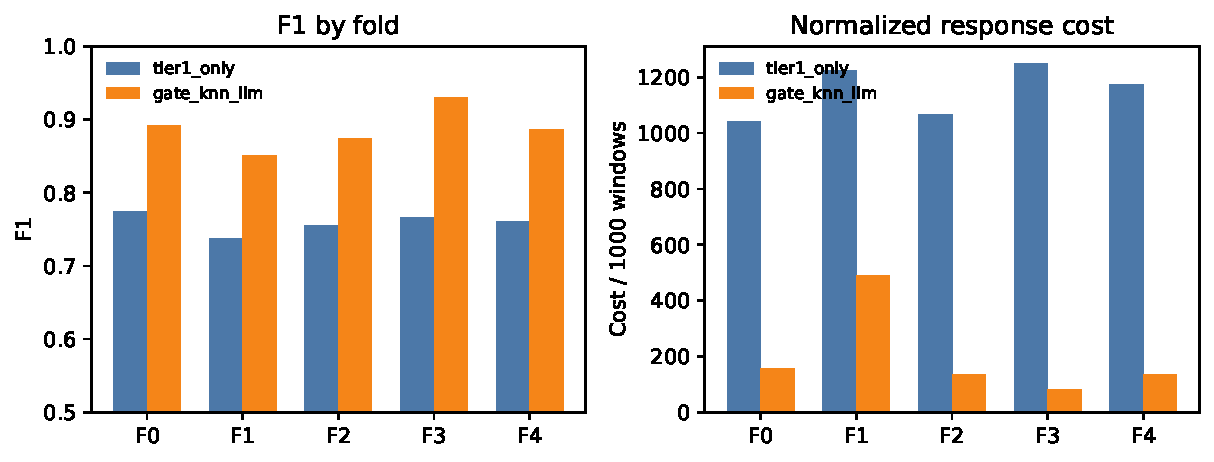
\includegraphics[width=\linewidth]{figures/cost_f1_per_fold.pdf}
\caption{Per-fold F1 and cost per $1000$ windows, \texttt{primary\_only} versus \texttt{gate\_knn\_llm} ($n{=}1000$/fold). Both metrics improve on every fold.}
\label{fig:costf1}
\end{figure}

\begin{table}[!t]
\centering
\caption{SisFall main protocol, five-fold mean$\pm$sample std ($n{=}1000$/fold, fall prevalence $0.433{\pm}0.004$), computed from the counts in Table~\ref{tab:confusion} before rounding. Paired intervals are fold-level percentile bootstrap ($10^4$ resamples, seed $42$); BCa intervals are F1 $[0.117,0.154]$, recall $[0.181,0.244]$, cost $[-1084,-834]$. The exact two-sided Wilcoxon $p$ is $0.0625$ for every metric (the minimum attainable with five pairs). Five overlapping folds make these intervals descriptive, not subject-level confidence intervals.}
\label{tab:meanstd}
\setlength{\tabcolsep}{4pt}
\begin{tabular}{lccccc}
\toprule
Mode & F1 & Recall & Prec. & Spec. & Cost/1k \\
\midrule
\texttt{primary\_only}
 & 0.759 & 0.759 & 0.760 & 0.815 & 1151 \\
 & {\scriptsize$\pm$0.014} & {\scriptsize$\pm$0.022} & {\scriptsize$\pm$0.032} & {\scriptsize$\pm$0.035} & {\scriptsize$\pm$93} \\
\addlinespace
\textbf{\texttt{gate\_knn\_llm}}
 & \textbf{0.887} & \textbf{0.977} & \textbf{0.813} & \textbf{0.828} & \textbf{200} \\
 & {\scriptsize$\pm$0.029} & {\scriptsize$\pm$0.037} & {\scriptsize$\pm$0.036} & {\scriptsize$\pm$0.039} & {\scriptsize$\pm$164} \\
\midrule
\multicolumn{6}{l}{\textit{Paired $\Delta$ (stack $-$ primary), 95\% percentile CI}} \\
\midrule
F1        & \multicolumn{5}{l}{$+0.128$ \quad $[0.117,\ 0.147]$ \quad 5/5 folds} \\
Recall    & \multicolumn{5}{l}{$+0.218$ \quad $[0.187,\ 0.248]$ \quad 5/5 folds} \\
Cost/1k & \multicolumn{5}{l}{$-951$ \quad\; $[-1079,\ -825]$ \quad 5/5 folds} \\
\bottomrule
\end{tabular}
\end{table}

\subsection{Controls}
The gate and retrieval components are evaluated using training-fold calibration
and subject-disjoint test folds. The complete code-free stack is retained only
when its decision reduces the validated cost objective; otherwise the frozen
detector prediction is used.

\subsection{External Evaluation}
KFall is retained as an external dataset for protocol validation. Because the
available evaluation is window-level and the code-free event-level report is
not yet complete, we do not make a cross-dataset superiority claim.

\subsection{Operating Cost}
The primary detector takes $8.56$\,ms per window; an escalated window takes $13.64$\,s, dominated by local decoding, and the mean is $6.37$\,s per window at escalation $0.468$ (Supplementary Table~S9, Fig.~\ref{fig:timeline}). Against a $50$\,ms stride, dense overlapping windows would require processing about $127\times$ faster than measured. RCDP in its current form is therefore an offline or near-real-time caregiver-triage layer that reviews candidate events within tens of seconds, not a real-time alarm or a pre-impact protection system.

\begin{figure}[!t]
\centering
\resizebox{\linewidth}{!}{% ---------------------------------------------------------------------
% Fig. 3 -- Latency budget of the two tiers on a logarithmic time axis.
% Marker values are the five-fold means of Table~\ref{tab:latency}
% (primary detector 8.56 ms; escalated path 13.63 s).
% Pure TikZ. Wrap with \resizebox{\linewidth}{!}{...} in main.tex.
% ---------------------------------------------------------------------
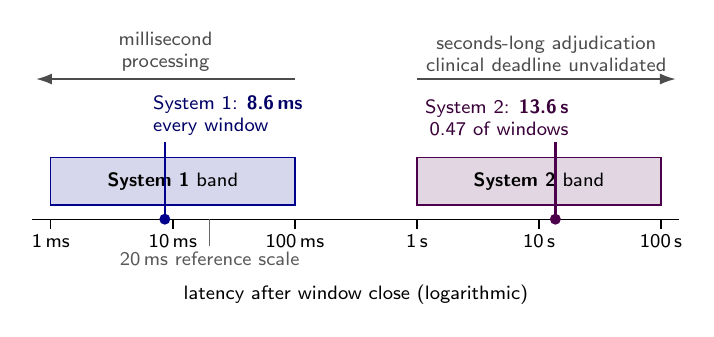
\begin{tikzpicture}[
  font=\footnotesize\sffamily,
  x=1.55cm, y=1cm,
  lbl/.style={font=\scriptsize\sffamily, inner sep=1.5pt},
  tick/.style={line width=0.5pt},
  arr/.style={-{Latex[length=2.0mm,width=1.4mm]}, line width=0.6pt}
]

% ---------- tier occupancy bands (x is log10 of time in ms) ----------
\fill[blue!55!black, fill opacity=0.16] (0.00,0.18) rectangle (2.00,0.78);
\draw[draw=blue!55!black, line width=0.5pt] (0.00,0.18) rectangle (2.00,0.78);
\node[lbl, align=center] at (1.00,0.48) {\textbf{System 1} band};

\fill[violet!60!black, fill opacity=0.16] (3.00,0.18) rectangle (5.00,0.78);
\draw[draw=violet!60!black, line width=0.5pt] (3.00,0.18) rectangle (5.00,0.78);
\node[lbl, align=center] at (4.00,0.48) {\textbf{System 2} band};

% ---------- time axis ----------
\draw[tick] (-0.15,0.00) -- (5.15,0.00);
\foreach \d/\t in {0/1\,ms, 1/10\,ms, 2/100\,ms, 3/1\,s, 4/10\,s, 5/100\,s}{%
  \draw[tick] (\d,0.00) -- (\d,-0.12);
  \node[lbl, anchor=north] at (\d,-0.14) {\t};
}

% ---------- external reference point ----------
\draw[line width=0.5pt, black!60] (1.301,0.00) -- (1.301,-0.34);
\node[lbl, anchor=north, text=black!65] at (1.301,-0.36)
  {20\,ms reference scale};

\node[lbl, anchor=north] at (2.50,-0.78) {latency after window close (logarithmic)};

% ---------- measured operating points ----------
\draw[line width=0.9pt, blue!55!black] (0.934,0.00) -- (0.934,0.98);
\node[circle, fill=blue!55!black, inner sep=1.4pt] at (0.934,0.00) {};
\node[lbl, anchor=south west, align=left, text=blue!40!black] at (0.80,1.00)
  {System 1: \textbf{8.6\,ms}\\every window};

\draw[line width=0.9pt, violet!60!black] (4.134,0.00) -- (4.134,0.98);
\node[circle, fill=violet!60!black, inner sep=1.4pt] at (4.134,0.00) {};
\node[lbl, anchor=south east, align=right, text=violet!45!black] at (4.28,1.00)
  {System 2: \textbf{13.6\,s}\\0.47 of windows};

% ---------- clinical budget annotations ----------
\draw[arr, black!70] (2.00,1.78) -- (-0.12,1.78);
\node[lbl, anchor=south, text=black!70, align=center] at (0.94,1.82)
  {millisecond\\processing};

\draw[arr, black!70] (3.00,1.78) -- (5.12,1.78);
\node[lbl, anchor=south, text=black!70, align=center] at (4.06,1.82)
  {seconds-long adjudication\\clinical deadline unvalidated};

\end{tikzpicture}
}
\caption{Processing timescales (five-fold means, Supplementary Table~S9); acquisition, queueing and caregiver response are excluded.}
\label{fig:timeline}
\end{figure}

% =====================================================================
\section{Discussion}
\label{sec:discussion}

\subsection{Where the Gain Comes From}
The modest aggregate difference is consistent with selective escalation under a
cost-sensitive objective, but the five-fold sample is too small for a strong
superiority claim. Whether deferral is worthwhile depends on deployment
latency, energy, and the relative cost of missed falls and false alarms.

\subsection{Comparison with Published Results}
Published SisFall figures are not directly comparable. Waheed \textit{et al.}~\cite{waheed2021ntfds} report $97.21\%$ accuracy for NT-FDS, while our detectors reach F1 $0.57$--$0.76$ on dense, trial-labelled, subject-independent windows. As Sec.~\ref{sec:labels} explains, label granularity rather than detector quality accounts for most of this gap; windowing, label assignment, subject splits and prevalence must match before results can be compared.

\subsection{Limitations}
\label{sec:limitations}
\emph{Label granularity.} Trial-level labels make per-window F1 a measure of
trial membership. Event-level metrics and free-living evaluation are required
before clinical translation.

\emph{Throughput and energy.} Escalation of $0.47$ (main) and $0.59$ (stress) at about $14$\,s per escalated window is roughly $127\times$ too slow for dense streaming on our hardware, and energy was not profiled. Event-triggered invocation, a quantised or distilled reasoner, or a cost-tuned classifier on the same evidence are the natural next steps.

\emph{Statistics.} Five overlapping folds limit inference; intervals are descriptive, and leave-one-subject-out analysis remains to be done.

\emph{Population and setting.} SisFall restricts older adults from the stress activities, the actions are simulated, and no caregiver-in-the-loop or free-living data were collected.

\emph{Reproducibility.} Local LLM decoding is not bitwise reproducible (paired runs differ by up to $0.022$ F1), and the mutable \texttt{mistral:latest} tag does not pin weights; digests must be recorded at release.

% =====================================================================
\section{Conclusion}
\label{sec:concl}

A confidence-gated decision layer around a frozen CNN--LSTM--Attention detector
produced a modest improvement in the verified SisFall aggregate (F1 $0.772$
versus $0.768$; cost $1079.6$ versus $1086.6$). The result is descriptive and
requires confirmation with event-level, free-living, and prospective evaluation
before clinical use.

% =====================================================================
\section*{Ethical and Data-Use Statement}
This retrospective study uses the public SisFall~\cite{sisfall2017} and KFall~\cite{kfall2021} datasets, whose collection ethics are documented by their authors; no new participant data were collected. Language-model inference ran locally. All actions were simulated; no alerts or interventions were issued. The cost ratio $\beta$ is an assumption, not a clinically validated utility.

\section*{Author Declarations}
\label{sec:authordecls}
Harshal Dharpure: conceptualization, methodology, software, investigation, data curation, analysis, writing, and visualization. Funding: none. The author declares no competing interests. Acknowledgments: none.

\section*{Data and Code Availability}
Table, figure and algorithm sources, verification scripts, per-fold confusion counts (\texttt{results\_text/}), locked YAML configurations (\texttt{configs/}) and prompt templates (\texttt{prompts/}) are provided at \url{https://github.com/harshalDharpure/agentic_elder_fall}. SisFall and KFall are available from their original authors. Supplementary material (\texttt{supplementary.pdf}) contains reproducibility notes (Section~S-I), full protocol settings (Section~S-II) and Tables~S1--S9.

% Reproducibility notes, protocol details and Tables S1--S9 are in
% supplementary.tex (compiled and uploaded separately).

\bibliographystyle{IEEEtran}
\bibliography{refs}

\end{document}
